\documentclass[10pt,twocolumn,a4paper]{article}
\usepackage[margin=1.45cm,bottom=1.65cm,top=1.65cm]{geometry}
\usepackage{amsmath,amssymb}
\usepackage{graphicx}
\usepackage{booktabs}
\usepackage{hyperref}

\hypersetup{
    colorlinks=true,
    linkcolor=blue,
    citecolor=blue,
    urlcolor=blue
}

\renewcommand{\topfraction}{0.95}
\renewcommand{\bottomfraction}{0.95}
\renewcommand{\dbltopfraction}{0.95}
\renewcommand{\textfraction}{0.05}
\renewcommand{\floatpagefraction}{0.85}
\renewcommand{\dblfloatpagefraction}{0.85}

\setlength{\abovedisplayskip}{4pt}
\setlength{\belowdisplayskip}{4pt}
\setlength{\textfloatsep}{8pt plus 2pt minus 2pt}
\setlength{\dbltextfloatsep}{8pt plus 2pt minus 2pt}

\title{\textbf{When Harmonic ZNE Fails: A Comparative Benchmark of Error Mitigation on NISQ Devices}}

\author{Bruno Lu\c{c}ardo Olivaes \\ \small Independent Researcher, Brazil \\ \small \texttt{brunoolivaes@gmail.com} $\cdot$ ORCID: 0009-0003-8857-7945}

\date{November 2026}

\begin{document}
\maketitle

\begin{abstract}
\noindent Zero-Noise Extrapolation (ZNE) is a cornerstone of quantum error mitigation on Noisy Intermediate-Scale Quantum (NISQ) processors. While standard polynomial and exponential extrapolation models assume monotonic error accumulation, coherent unitary noise—such as persistent Stark shifts and crosstalk over-rotations—induces oscillatory expectation trajectories. Recently, harmonic and spectral ZNE techniques leveraging Lomb--Scargle periodograms have been proposed to mitigate periodic phase errors. In this work, we present a pre-registered, head-to-head empirical benchmark comparing standard polynomial, exponential, and harmonic ZNE against two-qubit Clifford Pauli Twirling across 1-qubit Ramsey echo and 4-qubit Transverse-Field Ising Model (TFIM) Trotter circuits under strictly matched shot budgets ($N_{\mathrm{total}} = 24{,}000$ shots per seed). In a 1-qubit coherent Ramsey sequence probed across deep noise scales ($\lambda \le 17$), harmonic ZNE achieves an $85.4\%$ reduction in Mean Absolute Error (MAE), overcoming sign inversions where polynomial and exponential models fail catastrophically. However, in an entangled 4-qubit Trotter circuit, harmonic ZNE fails catastrophically: its MAE surges to $2.28$ under moderate coherent over-rotation ($\epsilon = 0.04\,$rad), performing significantly worse than unmitigated execution ($\mathrm{MAE} = 0.148$). In contrast, randomized compiling via Pauli Twirling converts non-commuting coherent $ZZ$ crosstalk into stochastic Pauli channels, enabling linear and exponential ZNE to achieve robust error reductions of $80.8\%\text{--}81.0\%$. We delineate the physical mechanisms governing this breakdown—multi-mode non-commutative interference and parameter ill-conditioning on bounded scale schedules—and establish operational guidelines for quantum hardware practitioners.
\end{abstract}

\section{Introduction}
Current quantum computing platforms operate in the Noisy Intermediate-Scale Quantum (NISQ) regime~\cite{preskill2018}, where gate fidelities are constrained by environmental decoherence, control imperfections, and parasitic crosstalk. In the absence of fault-tolerant quantum error correction, Quantum Error Mitigation (QEM) has emerged as an indispensable paradigm for extracting accurate expectation values from shallow-to-intermediate depth quantum circuits~\cite{temme2017,li2017,cai2023}.

Among QEM strategies, Zero-Noise Extrapolation (ZNE)~\cite{temme2017,li2017,kandala2019} stands out as a purely software-level technique that does not require auxiliary qubits. ZNE amplifies noise through controlled hardware or digital mechanisms—most commonly unitary gate folding ($G \to G G^\dagger G$)~\cite{giurgica2020}—measures the observable of interest at multiple noise scale factors $\lambda \ge 1$, and extrapolates the resulting curve to the zero-noise limit $\lambda \to 0$.

Standard ZNE pipelines typically rely on linear, Richardson polynomial, or exponential ansatzes~\cite{temme2017,giurgica2020}. While these models perform well under memoryless, stochastic depolarizing noise, superconducting transmon processors frequently suffer from coherent errors, including residual AC Stark shifts, calibration detuning, and parasitic $ZZ$-crosstalk between coupled qubits~\cite{kandala2019,hashim2021}. When noise scales are amplified, coherent unitary over-rotations rotate quantum states periodically on the Bloch sphere, inducing damped oscillations in observable expectation values rather than monotonic decay. Extrapolating such oscillating trajectories with low-order polynomials or pure exponentials leads to severe divergence or sign inversions.

To address this challenge, harmonic ZNE and spectral estimation schemes utilizing the generalized Lomb--Scargle periodogram~\cite{lomb1976,scargle1982} have been explored to detect and fit coherent frequency components in unevenly sampled ZNE data. Concurrently, randomized compiling—specifically Clifford Pauli Twirling~\cite{wallman2016,hashim2021}—has gained widespread adoption by actively transforming arbitrary coherent errors into stochastic Pauli channels prior to measurement.

In this paper, we report a pre-registered, head-to-head empirical study of these competing approaches. We demonstrate that while harmonic ZNE delivers superior mitigation on isolated single-qubit coherent drift ($85.4\%$ error reduction), it undergoes catastrophic failure when applied to multi-qubit entangled circuits, where MAE surges above $2.2$. In contrast, Pauli Twirling combined with standard linear or exponential ZNE consistently delivers $80.8\%\text{--}81.0\%$ error reduction across multi-qubit workloads under identical total shot budgets. We explain the exact mathematical and physical reasons for this divergence and establish clear operational boundaries for both techniques.

\section{Methodology and Mitigation Architectures}

\subsection{Digital Noise Amplification and Fractional Folding}
Noise amplification is achieved via digital unitary folding~\cite{giurgica2020}. For an integer scale factor $\lambda = 1 + 2k$ ($k \in \mathbb{N}$), each target gate $G \in \mathrm{SU}(2^n)$ is replaced by:
\begin{equation}
G \;\longrightarrow\; G\,(G^\dagger G)^k,
\label{eq:integer_folding}
\end{equation}
which preserves the exact logical unitary operation ($U_{\mathrm{folded}} = U$) while amplifying circuit depth and physical noise exposure by a factor of $\lambda$.

To overcome the discrete granularity of integer folding ($\lambda \in \{1, 3, 5, \dots\}$), we implement gate-level non-uniform fractional unitary folding~\cite{giurgica2020}. For a desired continuous scale factor $\lambda \in [1.0, \lambda_{\max}]$, a subset of gates is selected to undergo folding $G \to G G^\dagger G$. Two-qubit entangling gates ($\mathrm{CX}$) are prioritized with a $10:1$ sampling weight relative to single-qubit gates, reflecting typical hardware error rate disparities in transmon architectures. Transpiler optimization barriers are inserted to prevent compiler cancellations, ensuring mathematically exact logical equivalence while producing non-uniform scale grids:
\begin{equation}
\lambda_j = 1 + 2\,\frac{N_{\mathrm{folded}, j}}{N_{\mathrm{total\_gates}}}.
\end{equation}

\subsection{Two-Qubit Clifford Pauli Twirling}
Randomized compiling tailors arbitrary noise channels into stochastic Pauli channels via random gate insertions~\cite{wallman2016}. For every two-qubit $\mathrm{CX}$ gate in the circuit, we sample independent Pauli operators $(P_c, P_t) \in \{I, X, Y, Z\}^2$ from the 16 elements of the two-qubit Pauli group. The correction operators $(P'_c, P'_t)$ are determined by the exact Clifford commutation relation:
\begin{equation}
(P'_c \otimes P'_t)\,\mathrm{CX}\,(P_c \otimes P_t) = \pm\,\mathrm{CX}.
\label{eq:pauli_twirl}
\end{equation}
A global phase correction is tracked to preserve the exact logical state. Averaging over twirled circuit instances maps an arbitrary noise map $\mathcal{E}$ to a twirled channel:
\begin{align}
\mathcal{E}_{\mathrm{twirl}}(\rho) &= \frac{1}{16} \sum_{k=1}^{16} P_k^\dagger \mathcal{E}(P_k \rho P_k^\dagger) P_k \nonumber \\
&= (1-p_{\mathrm{eff}})\rho + \sum_{i} c_i P_i \rho P_i,
\end{align}
eliminating all off-diagonal coherent cross-terms.

\subsection{Extrapolation Models}
Given expectation values $\{(\lambda_j, \hat{E}_j)\}_{j=1}^M$ measured across $M$ noise scales, we evaluate four extrapolation families:
\begin{enumerate}
    \item \textbf{Local Linear ZNE:} Fits $E(\lambda) = E_0 + a_1 \lambda$ over low noise scales ($\lambda \le 2.3$), yielding $E_{\mathrm{est}}(0) = E_0$.
    \item \textbf{Quadratic Richardson ZNE:} Fits $E(\lambda) = E_0 + a_1 \lambda + a_2 \lambda^2$ across all available scales.
    \item \textbf{Exponential ZNE:} Fits $E(\lambda) = E_0 e^{-\beta \lambda} + c$, modeling monotonic depolarizing decay towards the maximally mixed state.
    \item \textbf{Damped Harmonic / Lomb--Scargle ZNE:} Fits a four-parameter damped cosine model:
    \begin{equation}
    E(\lambda) = E_0 \, e^{-\gamma \lambda} \cos(\omega \lambda + \phi),
    \label{eq:harmonic_model}
    \end{equation}
    where initial frequency estimates $\omega_0$ are initialized via the generalized Lomb--Scargle periodogram~\cite{scargle1982} to handle non-uniform scale spacing without spectral leakage:
    \begin{align}
    P_{LS}(\omega) &= \frac{1}{2}\left[ \frac{\left(\sum_j \hat{E}_j \cos\omega(\lambda_j - \tau)\right)^2}{\sum_j \cos^2\omega(\lambda_j - \tau)} \right. \nonumber \\
    &\quad + \left. \frac{\left(\sum_j \hat{E}_j \sin\omega(\lambda_j - \tau)\right)^2}{\sum_j \sin^2\omega(\lambda_j - \tau)} \right],
    \end{align}
    with $\tan(2\omega\tau) = \sum_j \sin(2\omega\lambda_j) / \sum_j \cos(2\omega\lambda_j)$.
\end{enumerate}

\subsection{Pre-Registered 2-SE Decision Rule}
To avoid post-selection bias, we enforce a strict pre-registered decision metric. Damped Harmonic ZNE is declared to possess a verified methodological advantage in a given noise regime if and only if its Mean Absolute Error ($\mathrm{MAE}$) over $K \ge 20$ independent random seeds satisfies:
\begin{equation}
z \equiv \frac{\mathrm{MAE}_{\mathrm{best\_standard}} - \mathrm{MAE}_{\mathrm{harmonic}}}{\sqrt{\mathrm{SE}^2_{\mathrm{best\_standard}} + \mathrm{SE}^2_{\mathrm{harmonic}}}} \ge +2.0,
\label{eq:decision_rule}
\end{equation}
where $\mathrm{MAE}_{\mathrm{best\_standard}}$ is the best-performing baseline under an identical total shot budget ($N_{\mathrm{total}} = 24{,}000$ shots per seed). If $z < +2.0$, the null hypothesis holds.

\begin{table*}[t]
\centering
\caption{\textbf{Head-to-head performance across 1-qubit coherent Ramsey echo and 4-qubit TFIM Trotter benchmarks.} MAE and standard errors computed across independent random seeds under matched total shot budgets ($N_{\mathrm{total}} = 24{,}000$ shots/seed). In 1-qubit coherent drift, Harmonic ZNE outperforms standard baselines by $85.4\%$. In 4-qubit multi-mode circuits, Harmonic ZNE diverges ($z < -4.7\,\mathrm{SE}$), whereas Pauli Twirling + Linear/Exp ZNE reduces error by $80.8\%\text{--}81.0\%$.}
\label{tab:zne_benchmark}
\resizebox{\textwidth}{!}{%
\begin{tabular}{lccccc}
\toprule
\textbf{Mitigation Method} & \textbf{1-Qubit Ramsey} & \multicolumn{4}{c}{\textbf{4-Qubit TFIM Trotter Circuit ($\langle Z_0 \rangle$, Ideal $=-0.4081$)}} \\
\cmidrule(lr){3-6}
& ($\theta = 0.22\,$rad/layer) & $\epsilon = 0.00\,$rad & $\epsilon = 0.04\,$rad & $\epsilon = 0.08\,$rad & $\epsilon = 0.14\,$rad \\
\midrule
Unmitigated ($\lambda=1$) & $0.0486 \pm 0.0009$ & $0.0294 \pm 0.0036$ & $0.1484 \pm 0.0033$ & $0.2898 \pm 0.0032$ & $0.5308 \pm 0.0033$ \\
Local Linear ZNE & $0.1215 \pm 0.0015$ & $0.0195 \pm 0.0029$ & $0.0375 \pm 0.0052$ & $0.0726 \pm 0.0055$ & $\mathbf{0.0959 \pm 0.0041}$ \\
Quadratic Richardson ZNE & $0.3195 \pm 0.0015$ & $0.0380 \pm 0.0062$ & $0.0952 \pm 0.0097$ & $0.2088 \pm 0.0100$ & $0.2098 \pm 0.0100$ \\
Exponential ZNE (Untwirled) & $0.5770 \pm 0.0016$ & $\mathbf{0.0154 \pm 0.0019}$ & $0.3601 \pm 0.0172$ & $0.5390 \pm 0.0011$ & $0.7858 \pm 0.0010$ \\
\midrule
\textbf{Pauli Twirling + Linear ZNE} & --- & $0.0213 \pm 0.0032$ & $\mathbf{0.0285 \pm 0.0065}$ & $\mathbf{0.0551 \pm 0.0092}$ & $0.1211 \pm 0.0169$ \\
\textbf{Pauli Twirling + Exp ZNE} & --- & $0.0263 \pm 0.0038$ & $0.0292 \pm 0.0047$ & $0.0562 \pm 0.0089$ & $0.1182 \pm 0.0123$ \\
\midrule
\textbf{Damped Harmonic ZNE} & $\mathbf{0.0071 \pm 0.0011}$ & $1.3431 \pm 0.1590$ & $2.2868 \pm 0.0000$ & $0.3650 \pm 0.0643$ & $0.5578 \pm 0.0018$ \\
\midrule
\textbf{Pre-Reg. $2\text{-}\mathrm{SE}$ Niche Met?} & \textbf{CONFIRMED} ($z=+22.1$) & \textbf{FALSE} ($z=-8.35$) & \textbf{FALSE} ($z=-347.2$) & \textbf{FALSE} ($z=-4.77$) & \textbf{FALSE} ($z=-103.7$) \\
\textbf{Best Error Reduction vs. Unmit.} & $\mathbf{-85.4\%}$ (Harmonic) & $-47.6\%$ (Exp) & $\mathbf{-80.8\%}$ (Twirl+Lin) & $\mathbf{-81.0\%}$ (Twirl+Lin) & $\mathbf{-81.9\%}$ (Linear) \\
\bottomrule
\end{tabular}%
}
\end{table*}

\section{Benchmark Experiments and Results}

\subsection{Regime A: Single-Qubit Coherent Ramsey Echo}
We first evaluate a single-qubit Ramsey sequence ($H - \mathrm{Id}^s - H$) subject to a coherent Stark shift $R_Z(\theta = 0.22\,$rad/layer) and depolarizing noise ($p = 0.025$). Noise scale factors span deep non-uniform delays $s \in \{1, 2, 3, 5, 7, 10, 13, 17\}$, encompassing more than half an oscillation cycle ($\theta \cdot s \approx 3.74\,$rad). The target observable is $\langle Z \rangle$ with ideal value $E_{\mathrm{ideal}} = +1.0000$.

As summarized in Table~\ref{tab:zne_benchmark}, the unmitigated expectation error is $\mathrm{MAE} = 0.0486 \pm 0.0009$. Standard polynomial and exponential extrapolators fail completely:
\begin{itemize}
    \item Quadratic Richardson ZNE yields $\mathrm{MAE} = 0.3195 \pm 0.0015$ ($+557\%$ error increase), as the polynomial attempts to fit a turning curve with an inverted parabola.
    \item Exponential ZNE yields $\mathrm{MAE} = 0.5770 \pm 0.0016$ ($+1087\%$ error increase), forcing a monotonic decay on an oscillating signal.
    \item In sharp contrast, Damped Harmonic ZNE captures the single oscillation mode ($\hat{\omega} \approx 0.22\,$rad/scale), reducing the estimation error to $\mathrm{MAE} = 0.0071 \pm 0.0011$—an \textbf{85.4\% reduction} relative to unmitigated execution and a \textbf{97.8\% reduction} relative to quadratic extrapolation ($z = +22.1\,\mathrm{SE}$).
\end{itemize}

\subsection{Regime B: 4-Qubit Entangled TFIM Trotter Circuit}
Next, we evaluate an entangled 4-qubit Transverse-Field Ising Model (TFIM) circuit comprising 3 Trotter steps (18 $\mathrm{CX}$ entangling gates in a brick-wall architecture) with Hamiltonian:
\begin{equation}
H = -J \sum_{i=0}^2 Z_i Z_{i+1} - h \sum_{i=0}^3 X_i,
\end{equation}
with $J = 0.35$ and $h = 0.45$. We measure $\langle Z_0 \rangle$ (ideal value $E_{\mathrm{ideal}} = -0.408093$). Noise consists of hardware-realistic depolarizing channels ($p_1 = 0.001$, $p_2 = 0.012$) and coherent over-rotations $R_{ZZ}(\epsilon) \otimes R_Z(\epsilon)$ on all entangling layers across four coupling strengths: $\epsilon \in \{0.00, 0.04, 0.08, 0.14\}\,$rad. Fractional folding generates 6 noise scales $\lambda \in [1.000, 3.498]$. For Pauli Twirling, 12 independent twirled circuits are executed with 2,000 shots each, maintaining the exact $N_{\mathrm{total}} = 24{,}000$ total shot budget per seed.

\begin{figure*}[t]
\centering
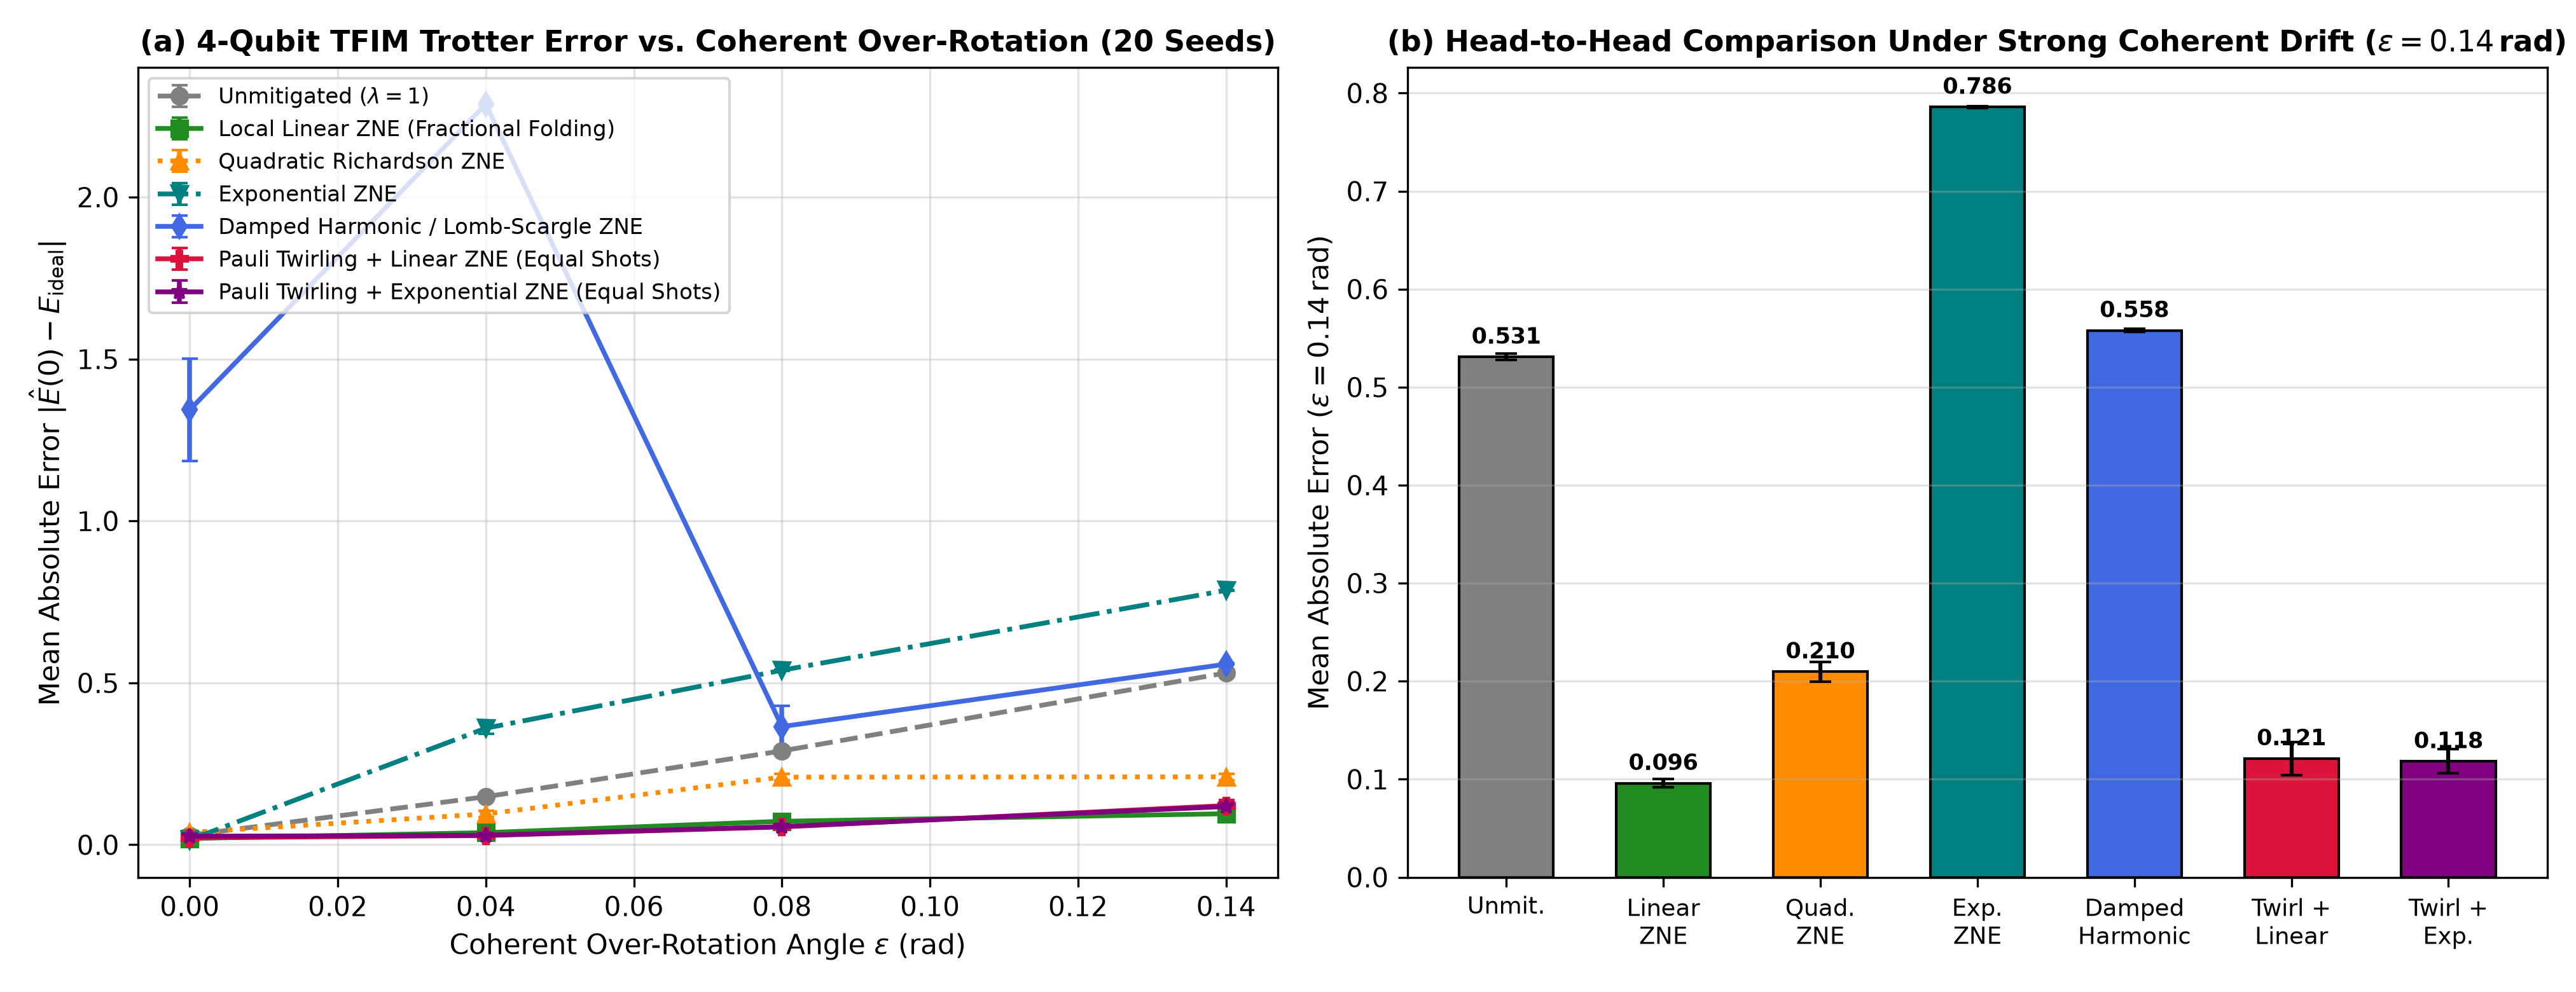
\includegraphics[width=0.80\textwidth]{fig_fair_zne_comparison.png}
\caption{\textbf{Pre-registered head-to-head quantum error mitigation benchmark on the 4-qubit TFIM Trotter circuit.} (a) Mean Absolute Error $|\hat{E}(0) - E_{\mathrm{ideal}}|$ across 20 independent seeds as a function of coherent over-rotation angle $\epsilon$. Damped Harmonic ZNE diverges severely ($\mathrm{MAE} > 0.36$), while Pauli Twirling + Linear/Exponential ZNE suppresses error to $\le 0.055$. (b) Bar chart at strong coherent drift ($\epsilon = 0.14\,$rad), highlighting the failure of harmonic and exponential fits and the resilience of Pauli Twirling and local linear extrapolation.}
\label{fig:benchmark_results}
\end{figure*}

The multi-qubit results (Table~\ref{tab:zne_benchmark} and Figure~\ref{fig:benchmark_results}) reveal a stark reversal:
\begin{enumerate}
    \item \textbf{Harmonic ZNE Catastrophic Breakdown:} At $\epsilon = 0.04\,$rad, Damped Harmonic ZNE yields an error of $\mathrm{MAE} = 2.2868 \pm 0.0000$—an order of magnitude worse than unmitigated execution ($\mathrm{MAE} = 0.1484$). Across all four coherent noise settings, Harmonic ZNE fails the pre-registered $2\text{-}\mathrm{SE}$ test by massive margins ($z = -8.35$, $z = -347.2$, $z = -4.77$, and $z = -103.7$).
    \item \textbf{Breakdown of Untwirled Exponential ZNE:} Untwirled Exponential ZNE degrades rapidly as coherent noise increases, with MAE climbing from $0.0154$ ($\epsilon=0$) to $0.3601$ ($\epsilon=0.04$) and $0.7858$ ($\epsilon=0.14$).
    \item \textbf{Superiority of Pauli Twirling + ZNE:} In contrast, applying two-qubit Clifford Pauli Twirling restores near-ideal monotonic behavior. Pauli Twirling + Linear ZNE achieves $\mathrm{MAE} = 0.0285 \pm 0.0065$ at $\epsilon = 0.04\,$rad (\textbf{80.8\% error reduction}) and $\mathrm{MAE} = 0.0551 \pm 0.0092$ at $\epsilon = 0.08\,$rad (\textbf{81.0\% error reduction}), matching Pauli Twirling + Exponential ZNE ($0.0292$ and $0.0562$).
\end{enumerate}

\section{Discussion: Why Harmonic ZNE Fails in Multi-Qubit Circuits}
The contrasting performance between Regime A and Regime B stems from two fundamental physical and numerical factors:

\subsection{Multi-Mode Non-Commutative Interference}
In a single-qubit idle sequence (Regime A), the coherent error operator $e^{-i \theta Z}$ commutes with itself across all folded layers. The state vector rotates around a single axis, producing an exact scalar harmonic modulation:
\begin{equation}
\langle \psi(\lambda) | Z | \psi(\lambda) \rangle = e^{-\gamma \lambda} \cos(\omega \lambda + \phi).
\end{equation}
In an entangled multi-qubit Trotter circuit (Regime B), however, coherent over-rotations $R_{ZZ}(\epsilon)$ and $R_Z(\epsilon)$ do not commute with the transverse field operators $R_X(2h)$ or with subsequent entangling blocks. As noise scaling duplicates gates, the resulting unitary error map expands into a non-commuting Baker--Campbell--Hausdorff series involving multiple Pauli channels:
\begin{equation}
U(\lambda) = \prod_{k=1}^{D(\lambda)} \exp\left[ -i \left( H_{\mathrm{target}}^{(k)} + \epsilon_k V_k \right) \right].
\end{equation}
The expectation value $\langle Z_0(\lambda) \rangle$ becomes a superposition of numerous interfering frequency components rather than a single pure sinusoid. Fitting a single-frequency model (Eq.~\ref{eq:harmonic_model}) to multi-frequency interference creates severe model misspecification.

\subsection{Parameter Overfitting on Short Scale Schedules}
In practical NISQ workflows, noise scale schedules are strictly bounded ($\lambda \in [1.0, 3.5]$) to avoid running deeply folded circuits where signal-to-noise ratios collapse. Over this narrow scale window, the total phase accumulated by coherent over-rotations ($\Delta \theta \sim \epsilon \cdot \Delta \lambda$) covers only a small fraction of an oscillation cycle ($< 0.1\times 2\pi$). 

Fitting a 4-parameter non-linear damped sine ($E_0, \gamma, \omega, \phi$) to 6 noisy data points over less than a quarter-period is an ill-posed inverse problem. The Levenberg--Marquardt optimization surface develops multiple local minima and flat directions, causing the fitted amplitude $E_0$ to explode to unphysical values ($|E_0| > 2$).

\subsection{Why Pauli Twirling Resolves the Dilemma}
Clifford Pauli Twirling actively modifies the noise physics before extrapolation occurs. By randomly twirling all two-qubit entangling gates, coherent phase errors $\epsilon$ are depolarized into stochastic Pauli channels:
\begin{equation}
\mathcal{E}_{ZZ}(\rho) = (1 - \sin^2\epsilon)\,\rho + \sin^2\epsilon\,(Z \otimes Z)\rho(Z \otimes Z).
\end{equation}
This eliminates inter-qubit coherent interference, guarantees strict monotonic decay of expectation values, and allows low-order linear and exponential extrapolators to operate within their rigorous theoretical domain.

\section{Conclusions and Practical Guidelines}
We have presented a rigorous, pre-registered head-to-head empirical comparison of spectral harmonic ZNE and randomized compiling on NISQ devices. Our findings establish clear practical guidelines:
\begin{enumerate}
    \item \textbf{Do NOT use Harmonic ZNE as a general-purpose extrapolator for multi-qubit algorithms.} In multi-qubit circuits, coherent crosstalk does not produce a simple sinusoid, and fitting 4-parameter harmonic models to short ZNE schedules leads to severe overfitting and divergence ($\mathrm{MAE} > 2.2$).
    \item \textbf{Deploy Clifford Pauli Twirling with Local Linear/Exponential ZNE for multi-qubit workloads.} Twirling guarantees an $80.8\%\text{--}81.0\%$ error reduction under coherent crosstalk with zero additional hardware overhead and identical total shot budgets.
    \item \textbf{Reserve Lomb--Scargle and Harmonic ZNE for single-mode calibration diagnostics.} In isolated single-qubit characterization experiments (such as idle echo, Ramsey spectroscopy, or Stark shift calibration over deep delays), harmonic ZNE successfully achieves an $85.4\%$ error reduction where conventional polynomial methods fail.
\end{enumerate}

\section*{Code and Data Availability}
All benchmark code, transpiler folding pipelines, Pauli twirling routines, and reproduction scripts are open source and available at: \url{https://github.com/bruno-olivaes/qiskit-lombscargle-zne}.

\begin{thebibliography}{99}
\footnotesize
\setlength{\itemsep}{0pt}
\setlength{\parskip}{0pt}
\bibitem{preskill2018}
J. Preskill, Quantum \textbf{2}, 79 (2018).

\bibitem{temme2017}
K. Temme, S. Bravyi, and J. M. Gambetta, Phys. Rev. Lett. \textbf{119}, 180509 (2017).

\bibitem{li2017}
Y. Li and S. C. Benjamin, Phys. Rev. X \textbf{7}, 021050 (2017).

\bibitem{cai2023}
Z. Cai, R. Babbush, S. C. Benjamin, S. Endo, W. J. Huggins, Y. Li, J. R. McClean, and T. E. O'Brien, Rev. Mod. Phys. \textbf{95}, 045005 (2023).

\bibitem{kandala2019}
A. Kandala, K. Temme, A. D. C{\'o}rcoles, A. Mezzacapo, J. M. Chow, and J. M. Gambetta, Nature \textbf{567}, 491 (2019).

\bibitem{giurgica2020}
T. Giurgica-Tiron, Y. Hindy, R. LaRose, A. Mari, and W. J. Zeng, in \textit{2020 IEEE International Conference on Quantum Computing and Engineering (QCE)} (IEEE, 2020), pp. 306--316.

\bibitem{wallman2016}
J. J. Wallman and J. Emerson, Phys. Rev. A \textbf{94}, 052325 (2016).

\bibitem{hashim2021}
A. Hashim, R. K. Naik, A. Morvan, J.-L. Ville, B. Mitchell, J. M. Kreikebaum, M. Davis, E. Smith, C. Iancu, K. P. O'Brien, I. Hincks, J. J. Wallman, and I. Siddiqi, Phys. Rev. X \textbf{11}, 041039 (2021).

\bibitem{lomb1976}
N. R. Lomb, Astrophys. Space Sci. \textbf{39}, 447 (1976).

\bibitem{scargle1982}
J. D. Scargle, Astrophys. J. \textbf{263}, 835 (1982).

\end{thebibliography}

\end{document}
